% !TeX program = lualatex
\documentclass{article}

\usepackage{hyperref}
\hypersetup{
	colorlinks = true,
	linkcolor = blue,
}
\usepackage{enumitem}
\newlist{steps}{enumerate}{1}
\setlist[steps, 1]{label = \arabic*:}

\usepackage{graphicx}

\usepackage{listings}
\usepackage{color}

\definecolor{dkgreen}{rgb}{0,0.6,0}
\definecolor{gray}{rgb}{0.5,0.5,0.5}
\definecolor{mauve}{rgb}{0.58,0,0.82}


\lstset{frame=tb,
	language=Java,
	aboveskip=3mm,
	belowskip=3mm,
	showstringspaces=false,
	columns=flexible,
	basicstyle={\small\ttfamily},
	numbers=none,
	numberstyle=\tiny\color{gray},
	keywordstyle=\color{blue},
	commentstyle=\color{dkgreen},
	stringstyle=\color{mauve},
	breaklines=true,
	breakatwhitespace=true,
	tabsize=3
}

\usepackage{amsmath}

\begin{document}

\title{AP Computer Science Manual}
\author{Brandon Waller | brandonw@live.com}

\maketitle

\tableofcontents

\section{Purpose}
Reading and understanding should guarantee at least a 4 on the ap exam and a 90\% chance of getting a 5. This is also an excuse for me to practice \LaTeX. 

\section{Introduction}
to score well on the AP exam, you will need to have a grasp of the basics of Java, a programming language that is rarely used any more, but the college board for some reason won't switch to Python. 

\subsection{Running Java Programs}
\textbf{note:} Skip this section until you are ready to run Java programs\\
To run Java programs, you will either need to install a Java IDE (Integrated Development Environment) on PC/Linux/Max , or use a terminal compiler on Linux or Mac.

\subsubsection{BlueJ}
When I took the class, we all used BlueJ, a free Java IDE. You can download it from this \href{https://www.bluej.org/}{Link.} you may also need to download a \href{http://www.oracle.com/technetwork/java/javase/downloads/jdk8-downloads-2133151.html}{JDK} (Java Development Kit)

\subsubsection{Linux/Unix Terminal}
Run the following commands in the Terminal to run and compile .Java files:
\begin{steps}
	\item sudo apt-get install openjdk-8-jre
	\item sudo apt-get install default-jdk
\end{steps}
To run and compile a file with the name \textbf{helloworld.java}:
\begin{steps}
	\item javac helloworld.java
	\item java helloworld
\end{steps}
\begin{figure}[h]
	\centering
	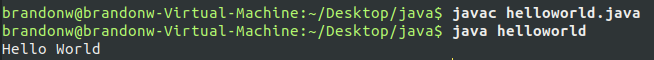
\includegraphics[width=0.7\linewidth]{runningjavafileonterminal}
	\caption[]{Running a .java file from the terminal}
	\label{fig:runningjavafileonterminal}
\end{figure}
Additionally, you may want to learn how to use a terminal text editor such as vim or emacs to edit files.
\subsubsection{The .java file}
Java programs are written in a .java file that is interpreted by the java compiler to execute the instructions.
\begin{figure}[h]
	\centering
	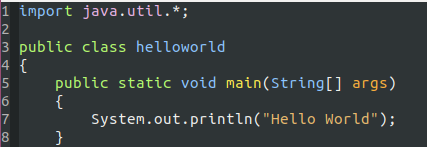
\includegraphics[width=0.7\textwidth]{helloworld}
	\caption[]{Hello World Java program}
	\label{fig}
\end{figure}
Features of this file
\begin{steps}
	\item line 1: importing java.util.*, a file that include additional Java functions
	\item line 3: class declaration, puclic class followed by the file name
	\item line 5: The main method. The set of instructions that are ran when by the executable after compiling
	\item line 7: Java functions
\end{steps}
There are many more things that go into .java files. These are just a few.

\section{Java Basics}
\subsection{Introduction}
Java is an object-oriented programming language developed by Sun Microsystems in 1995, and is the main language for Android app development. \\
This section will cover the basics of Java including data types, operations, loops, and control structures.
\subsubsection{bits}
In computers, data is stored in bits that can either have a value of 1 or 0. Each data type is defined by the number of bits consumed by the data type, and by the way the bits are interpreted by the compiler. For example, the number $23$ in 8-bit binary is $00010111$ and the number $-23$ is stored as $11101001$. This will be discussed later, but when converted to decimal $11101001$ is $233$. Depending on the data type, the compiler will either decide to make that number $-23$ or $233$.
\subsection{Data Types}
Data types are the classifications given to variables/data. Unlike other languages such as Python and MATLAB, java requires the programmer to explicitly state the data type for a variable, making this section more important to know when programming in Java.
\subsubsection{Primitives}
Primitives are the basic Java data types used to store variables in memory. They are as follows:
\begin{steps}
	\item byte: 8-bit signed data type (value $[-127,127]$) used for applications where memory space is limited 
	\item int: 32-bit integer value that can positive and negative value
	\item float: 32-bit decimal value
	\item double: 64-bit decimal value, can hold more data than a float
	\item char: 16-bit single character
	\item boolean: stores either true or false
\end{steps}

\subsubsection{Declaring and Converting Primitives}
Declaring a primitive in Java:
\begin{lstlisting}
	int x = 3;
	byte y = 127l
	double z = -12.34567;
	booean bool = true;
	char a = 65;
	char b = 'A';
	//both a and b have the same value. Each character is
	//mapped to a number 
\end{lstlisting}
The left side of the $=$ sign is the data type followed by the variable's name. On the right, is the value of the data type.
Sometimes, you will want to convert one primitive to another, for example rounding a a double to whole number. This is how you would do it. This uses if statements which will be discussed later:
\begin{lstlisting}
	double x = 2.6;
	int x_whole = (int) a;//converts a to an int by removing the portion after the decimal point
	if(x - x_whole >= 0.5)//if the decimal is greather than or equal to 0.5
		x = x_whole + 1;//round up by removing the decimal and adding 1
	else
		x = (int) x;//rounding down, simply remove the decimal
\end{lstlisting}

\subsubsection{Objects}
Objects are other data types that are either defined by the Java language, or can be created by the user (new primitive types cannot be created by the user). Additionally, unlike primitives, functions can be called on objects, potentially modifying their values.\\
Some common objects defined by the Java language are
\begin{steps}
	\item  String: A group of characters
	\item Integer
	\item Double
\end{steps}
\textbf{note: Objects start with capital letters while primitives start with lower case}
\subsubsection{Declaring Objects}
The syntax is slightly different for the declaration of objects
\begin{lstlisting}
	Integer j = 20;
	String str = "the is the text for the string";
	String s = new String();
	s = "this is the text for String s";
\end{lstlisting}
\textbf{The syntax for creating an instance for a user defined object will be a little different}
One of the defining features that distinguishes primitives from objects is that you can call functions on onbjects:
\begin{lstlisting}
	String s = "abcd";
	System.out.println(s.lnegth());//output = 4
\end{lstlisting}
Because String is an object, you can call the function \textbf{.length()} on it.
\subsubsection{Arrays and the ArrayList}
Arrays are a group of variables that can be individually addressed and have a set size. They are useful for storing data of fixed length. Here is how you declare and use an array:
\begin{lstlisting}
//Methods for declaring a new array
int[] i = new int[10];
int[] j = {1,2,3};
String[] s = new String[3];
String[] t = {"a", "b", "c"};
//Assigning values to an array
i[0] = 1;
i[1] = 2;
i[9] = 10;
s[0] = "abc";
//j and t already have values and are both size 3
//getting the length of an array
s.length;
i.length;
//accessing data from an array
i[1];
t[2];
j[1] + i[9];
\end{lstlisting}
\textbf{note: Java, like any well written programming language starts its arrays at 0.}

The ArrayList, unlike the array, does not have a define length. However, primitives cannot be stored in an ArrayList
\begin{lstlisting}
//Basic syntax for creating an ArrayList: ArrayList<object type> name = new ArrayList<object type>();
ArrayList<String> strings = new ArrayList<String>();
ArrayList<Integer> integers = new ArrayList<Integer>();
//adding data to ArrayList
strings.add("abc");//add "abc" to index 0
strings.add("def");//add "def" to index 1
strings.add("ghi");
integers.add(1);
integers.add(2);
integers.add(3);
integers.add(0,4);//add 4 to index 0, shifting each element in the ArrayList forward
//accessing the data in an ArrayList 
strings.get(0);//abc
strings.get(2);//ghi
integers.get(3);//3
//removing from an array list
strings.remove(0);//remove index 0 from the ArrayList and shift the rest of the list back
strings.get(0);//def
\end{lstlisting}
\subsection{Operations}
For the early stages of the class, you will mainly be staying within the \textbf{main()} function. This section will cover some of the basic operations you can do.
\subsubsection{System.out.print(String)}
System.out.print (and System.our.println()) are functions for displaying information to the console window. when using println(), subsequent text will be placed on a new line.
\begin{lstlisting}
System.out.print("Hello");
System.out.print("World");
System.out.println("Hello ");
System.out.println("World");
\end{lstlisting}
\begin{figure}[h]
	\centering
	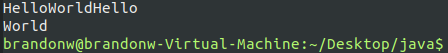
\includegraphics{consolewindowprint1}
	\caption{Console Window Output}
\end{figure}
Variables can be included in print statements. Each variable is separated by a $+$. When the variables are replaced by their value, they are included without a space.
\begin{lstlisting}
String a = "a";
String b = "c";
String c = "c";
int x = 123;
System.out.println(a + b + c + x);
System.out.println("abc123");
System.out.println(a + " " + b + " " + c + x);
System.out.println("a b c 123");
\end{lstlisting}
\begin{figure}[h]
	\centering
	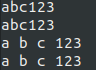
\includegraphics{consolewindowprint2}
	\caption{Console window output}
\end{figure}
Adding a " " between variables will but a space in the output.

\subsubsection{Mathematical Operations}
Java includes many mathematical operations, and many more can be added with the 
\textbf{java.math} package. 
\begin{lstlisting}
int x = 3, y = 5;
x + y;//8
x - y;//-2
x * y;//15
x / y;//0
squrt(4);//2
sin(0);//0
\end{lstlisting}
\textbf{Why is the result of x/y 0?}\\
When two integers are divided, the result is stored as an integer. The result of dividing 3 and 5 is 0.6, which is stored as the integer 0. These are correct ways to divide integers and store the result as a double:
\begin{lstlisting}
int x = 3, y = 5;
double z;
z = x/(double)y;//casting y as a double will result in a double result
z = 3/5.; z = 3/5.0;
//These implementations do not work:
z = (double)x/y; z = 3.0/5;
//The denominator must be a double for the result of division to be a double
\end{lstlisting}

\subsubsection{Modulo}
The modulo is an operations similar to division, but the output is the remainder. The modulo operation is represented by the \% sign. For example, $22~\%~10 = 2$ because $ \frac{22}{10} = 2r2$

\subsection{Control Structure}
Control Structure is using boolean expressions to control if/when code is ran. 
\subsubsection{Boolean Operations}
The boolean operations are as follows:

\begin{align*}
	 >  &: \text{Greater than}\\
	 >= &: \text{Greater than or equal to} \\
	 <  &: \text{Less than}\\
	 <= &: \text{Less than or equal to}\\
	 == &: \text{Equal to} \\
	 != &: \text{Not equal to} \\
	 !  &: \text{Not/Negation. Converts a boolean to the opposite value.}\\
	 \&\& &: \text{and. Comparison of two booleans. True if and only if both conditions are true.}\\
	 || &: \text{or. Comparison of two booleans. If either is true, the or operation results in true}
\end{align*}
These operations are used to compare values and other booleans and result in a boolean. Here are some examples:
\begin{lstlisting}
true == false;//false
true == true;//true
false == false;//true
1 >= 0;//true
1 > 1;//false
!true;//false
!false;//true
!(true || false);//false
!(!(true)||false) && true;//true
\end{lstlisting}

\subsubsection{If,If-Else, Else}
These three operations are the main three for controlling functions using boolean conditions. The basic syntax for this type of control is:
\begin{lstlisting}
if(/*condition*/)
	//do something
//optional
else if(/*some other condition*/)
	//do soemthing else
.....
else
	//If none of the conditions are true, run this code
\end{lstlisting}
In this type of statement, only one set of code will run regardless of how many are true. For example:
\begin{lstlisting}
int x = 8;
if(x == 10)
	System.out.pritln("The value of x is 10");
else if(x % 2 == 0)
	System.out.println("x is an even number");
else if(x >= 5)
	System.out.println("x is greater than or equal to 5");
else
	System.out.println("None of the conditons are true");
\end{lstlisting}
The result of this code will be \textbf{x is an even number}. Although it is true that x is >= 5, that line will not be executed because the rest of the if-else statement is passed after one of the conditions is true. A way to implement this function so that all the applicable lines are executed is:
\begin{lstlisting}
int x = 8;
if(x == 10)
	System.out.pritln("The value of x is 10");
if(x % 2 == 0)
	System.out.println("x is an even number");
if(x >= 5)
	System.out.println("x is greater than or equal to 5");
if(!(x == 10 || x % 2 == 0 || x >=5))
	System.out.println("None of the conditons are true");
\end{lstlisting}
If the last line was kept as \textbf{else} then the code would be executed if x < 5 is true, even if x is even, or equal to 10.

\subsubsection{Loops}
Loops are a control structure that allows lines of code to be repeated many times, saving time when writing code, and allowing programs to be more flexible. There are two types of loops: \textbf{for} and \textbf{while} loops. They are both fundamentally the same, but have different syntax.\\
The first type of loop is the \textbf{for} loop. It consists of declaring a variable, a condition, and the increment. When a for loop is created, a variable is given a variable, and it is compared against the condition. If the condition is true, then the code inside the loop runs. After, the variable is changed by the increment, and the process is repeated. Here is a for loop and a description of each step:
\begin{lstlisting}
for(int i = 0; i < 3; i++)
{
	System.out.print("*");//The College Board loves printing *'s
}
\end{lstlisting}
\begin{steps}
	\item declare the variable \textbf{i} with the value 0
	\item evaluate i < 3 which results in true
	\item output: *
	\item evaluate: i++ (the ++ and -- operation increase/decrease the variable by 1 respectively)
	\item evaluate: i < 3 which results in true
	\item output: **
	\item evaluate: i++
	\item evaluate: i < 3 which results in true
	\item output: ***
	\item evaluate: i++
	\item evaluate: i < 3 which results in false (3 < 3 is false)
\end{steps}
In a while loop, the variable is declared outside the loop, and the increment is inside the loop, meaning that you can change the increment and any time, not just at the end of the body of the loop. Here is an equivalent implementation using a while loop:
\begin{lstlisting}
int i = 0;
while(i < 3)
{
	System.out.println("*");
	i++;
}
\end{lstlisting}
\subsubsection{Nested Loops}
Loops can appear inside other loops:
\begin{lstlisting}
for(int i = 0; i < 3; i++)
{
	for(int j = i; j < 3; j++)
	{
		System.out.print("*")
	}
	System.out.println();
}
\end{lstlisting}
Output:
\begin{align*}
***\\
**\\
*
\end{align*}

Loops with arrays and ArrayLists
\begin{lstlisting}
ArrayList<Integer> integers = new ArrayList<Integer>();
int[] ints = new int[10];
//Using a for loop to set values for in ints and integers
for(int i = 0; i < ints.length; i++)
{
	integers.add(i);
	ints[i] = i;
}
//integers and ints have the values 0...9
//increase each value by 1 
for(int i = 0; i < integers.size(); i++)
{
	integers.set(i, integers.get(i) + 1);//set the element at index i to the value at index i + 1
	ints[i] += 1;
}
/*
**There is also the for-each loop that can access the data within an array list or array, but cannot change it
*/
for(int x : ints)
	System.out.print(x);
//this is equivilant to the following
for(int i = 0; i < ints.length; i++)
{
	int x = ints[i];
	System.out.print(x);
}
\end{lstlisting}

\subsection{Questions}
\textbf{Create the following pattern by editing the code provided:}
\begin{align*}
****\\
****\\
**\\
**\\
****\\
****
\end{align*}
\begin{lstlisting}
int i = 0;
while(i < 6)
{
	for(int j = 0; /*implemnt condition*/; j++)
	{
		/*
			Implement body
		*/
	}
	i++;
}
\end{lstlisting}
\textbf{Evaluate the following given that t = true and f = false:}
\begin{steps}
	\item !((t || f) == f)
	\item !(!(t \&\& f) == t)
	\item ((f == f) != (5 > 4)) || (3 < 5)
	\item (f == (!f || (5 < (8 \% 3))))
	\item 5/3. == 5/3
	\item 5./3 == 5/3
\end{steps}
\textbf{Create a for loop that will reverse the order of an array}
before: i = [1,2,3,4,5]
after: i = [5,4,3,2,1]
\begin{lstlisting}
//code for swapping data without creating a new variable
int[] x = new int[2];
x[0] = 1;x[2] = 2;
x[0] = x[0] + x[1];//3
x[1] = x[0] - x[1];//3 - 2 = 1, x[1] is now equal to the old value of x[0]
x[0] = x[0] - x[1];//3 - 1 = 2, x[0] is now equal to the old value of x[1]
\end{lstlisting}
\section{Classes and Objects}

Classes allow you to create your own object types that can be changed by user defined functions. Each .java file can define one object. Here is a .java file for an on object called \textbf{Obj}:
\begin{lstlisting}
import java.util.*;

public class Obj
{
	private int x,y;//private variables
	public obj(int x, int y)//constructor
	{
		this.x = x; this.y = y;
	}
	//get methods
	public int getX()
	{
		return x;
	}
	public int getY()
	{
		return y;
	}
	//set methods
	public void setX(int x)
	{
		this.x = x;
	}
	public void setY(int y)
	{
		this.y = y;
	}
	//main
	public static void main(String[] args)
	{
		Obj o = new Obj(3, 5);
		o.getX();//3
		o.getY();//5
		o.setX(10);
		o.getX();//10
	}
}
\end{lstlisting}
components of this class:
\begin{steps}
	\item Private variables: Variables that cannot be accessed by normal means. Methods can be written to access private variables
	\item Constructor: A function that is called when creating a new instance of the object. An onject may have many different constructors
	\item Get methods: Methods that return the value of private variables
	\item Set methods: Methods that set the value of private variables
\end{steps}

\subsection{Why use objects?}
\begin{steps}
	\item Code reuse: Several instances of the same object can be created to save time and make more organized code.
	\item Variable scope: Variables outside of objects cannot have their value changed by other functions. Variables inside objects can through set and other methods
	\item Control: Set ways for accessing the data within an object
\end{steps}
\end{document}
